%% This is an example first chapter.  You should put chapter/appendix that you
%% write into a separate file, and add a line \include{yourfilename} to
%% main.tex, where `yourfilename.tex' is the name of the chapter/appendix file.
%% You can process specific files by typing their names in at the 
%% \files=
%% prompt when you run the file main.tex through LaTeX.

\begingroup%
\makeatletter%
\cleardoublepage%
\let\newpage\relax%
\let\clearpage\relax%
\vspace*{\fill}%
\vspace*{\dimexpr-50\p@-\baselineskip}% Remove the initial
%% -default- 50pt gap (plus 1 line) 
\chapter{Introduction}
\label{chap1}
\vspace*{\fill}%
\endgroup%

\clearpage
Much of chemical oceanography and organic geochemistry is concerned in some way with the very small fraction of fixed organic matter that is preserved in sediments at the bottom of the sea. This organic matter must survive various destructive forces in the surface ocean and water column, all of which have the thermodynamic advantage. On timescales of millennia --- i.e., within the faster of Earth's two carbon cycles (Falkowski, 2014) --- the burial of the reduced carbon contained in this organic matter is the primary source (in a mass-balance sense) of atmospheric oxygen. On longer timescales, an even smaller fraction of this carbon survives to enter the Earth's lithosphere, which contains a massive $15\times10^6$ Pg of carbon (Petsch, 2014). Because of the importance of this small fraction of organic matter, it is no surprise that the various processes which determine its size and nature have been the subject of continual scientific investigation for centuries.

Although the ocean's biological pump was not formally defined as such until the late 20th century (Volk and Hoffert, 1985; Broecker, 1981), the hypothesis that the atmospheric and terrestrial compartments of the earth system could be connected in some meaningful way through chemical reactions in the oceans and hydrosphere first formally appeared in the late 19th century in the work of Arrhenius (1896), Chamberlin (1898), and contemporaries (Sundquist and Ackerman, 2014).\textsuperscript{1}\let\thefootnote\relax\footnote{{\setlength{\parindent}{0pt}\textsuperscript{1} The more fundamental notion that the chemical constituents of seawater could be subject to cycles of input and output orignated with Perrault (1674), who drew on the work of the Greek philosophers (Mottl and Elderfield, 2014). A wonderful history of biogeochemistry, with attention to the many early scientific contributions that shaped the discipline's development, can be found in Gorham (1991).}} In 1924, Vernadsky made one of the earliest attempts to quantify the sizes of the various carbon reservoirs that are connected through this hydrological nexus. His estimate of the size of the lithospheric carbon reservoir, $8\times10^{16}$ metric tons (or $8\times10^7$ Pg), was remarkably close to modern estimates. Vernadsky's other major contribution was, of course, to propose the term \emph{biogeochemistry} to describe the transfers of energy and carbon between these reservoirs, and the effects of and consequences for biota within each. Among the first modern oceanographers to investigate the transfer of energy and carbon between various biogeochemically distinct regions of the ocean were Dugdale and Goering (1967) and Eppley and Peterson (1979), who introduced the concepts of new versus regenerated primary production in the surface ocean and then established the importance of the former for the export of particulate matter to the deep sea, respectively.

Among modern geochemists and chemical oceanographers whose primary domain is these sinking marine particles and marine sediments, scientific inquiry into the fate of organic matter originating in the surface ocean has often been framed in terms of remineralization (i.e., oxidation by one or more terminal electron acceptors) or selectivity (or non-selectivity) in the preservation of certain of its components (e.g., Berner, 1981; D. Krom and A. Berner, 1981; Hedges et al., 2001; Keil et al., 1994; Middelburg, 1989; see also Figure 1). Of particular interest to chemical oceanographers and geochemists in this regard are the lipids of marine plankton, biochemicals whose taxonomic specificity and functional diversity make them uniquely suited for use as biomarkers of particular taxa or biogeochemical processes (Close et al., 2013; Pearson, 2014; Rontani et al., 2012; Sturt et al., 2004; Wakeham et al., 1997). Lipids and their many oxidation products are equally useful as indicators of various processes and phenomena in living or senescent biomass (Hunter et al., 2015; Van Mooy et al., 2006; Van Mooy et al., 2009; Vardi et al., 2012). Implicit in the use of these molecules as biomarkers is the recognition that they may be shaped and transformed by diverse catabolic and diagenetic processes in the water column and (when persisting for sufficient time) in sediments (Killops and Killops, 2005).

It is when one moves closer to the ocean's surface --- as I have in the course of researching and writing this thesis --- that a nuanced consideration of the various biological and abiotic processes which can contribute to the remineralization of organic matter is often simplified to a balance between aerobic respiration and primary production, i.e.
\begin{equation}
\begin{aligned}
  \text{GPP}=\text{NCP}+\text{GR}
\end{aligned}
\end{equation}
where GPP is gross primary production, NCP is net community production, and GR is gross (community) respiration. In the vast majority of cases, this is a logical and very useful simplification: The surface ocean is where photosynthesis takes place, and aerobic respiration by heterotrophic bacteria is the ultimate sink for particulate (Giering et al., 2014; Ploug and Grossart, 1999) and dissolved (Ar\'{i}stegui et al., 2002; Carlson and Ducklow, 1996) organic matter in virtually every major marine ecosystem (though, the state of the balance between the two processes is still hotly debated; e.g., del Giorgio and Duarte, 2002; del Giorgio et al., 1997; Ducklow and Doney, 2013; le B. Williams, 1998).

Yet, there is considerable evidence that select other processes which can degrade or remineralize organic matter may be significant in shaping both trophic balance in surface and pelagic ecosystems and the rate at which sinking marine particles are lost during their transit to the seafloor. First, several studies have shown that photochemical processes can directly oxidize some fractions of dissolved organic carbon (DOC) to inorganic forms at scales which are globally significant (Miller and Zepp, 1995; Mopper and Kieber, 2002; Mopper et al., 1991). This direct photochemical oxidation of DOC to CO$_2$ represents the extreme case in which a process other than aerobic respiration acts as the immediate and ultimate sink for fixed organic matter. The more profound significance of non-respiratory processes for ocean biogeochemistry can be seen in the many instances in which aerobic respiration or another biologically mediated oxidation reaction remains the ultimate sink for organic matter but one of these processes fundamentally facilitates the remineralization.

This is the case with photochemical degradation of dissolved organic matter: In many instances, while only a small fraction of DOC is directly oxidized to CO$_2$, photochemical reactions make a more significant additional fraction available to bacteria by reducing complex, often recalcitrant molecules to smaller labile components (Kieber et al., 1989; Zafiriou et al., 2003). This more labile DOC can then be remineralized at rates that far exceed those achievable in the absence of photochemistry. The significance of indirect contributions to rates of remineralization by non-respiratory processes can also be seen in increasing evidence from sinking marine particles. While aerobic respiration by free-living and particle-attached bacteria remains the ultimate sink for marine snow, other processes such as ``sloppy feeding'' or mechanical disaggregation by zooplankton may prepare organic material for heterotrophic metabolism by rendering it more labile (Grossart et al., 2007; Stemmann et al., 2004). These processes can, in some instances, be highly significant (Giering et al., 2014). Photochemical processes may also act on particulate organic carbon in a manner similar to DOC (Rontani et al., 2012).

While the chapters in this thesis are largely the product of a number of separate research projects, they are therefore joined together by two primary themes: Each focuses on a process or processes which augment or facilitate the degradation of organic matter by respiration, and, in two instances, lipids and their oxidation products are explored as biomarkers to assess processes' significance and magnitude. In all cases, I have sought to combine oceanographic field experiments and traditional geochemical analyses with novel modeling and computational approaches. While lipids are the central focus of this work in a geochemical sense, the projects in this thesis span multiple domains of chemistry and depth within the ocean (\autoref{fig:c1n1}).

\begin{figure}[t]
\centering
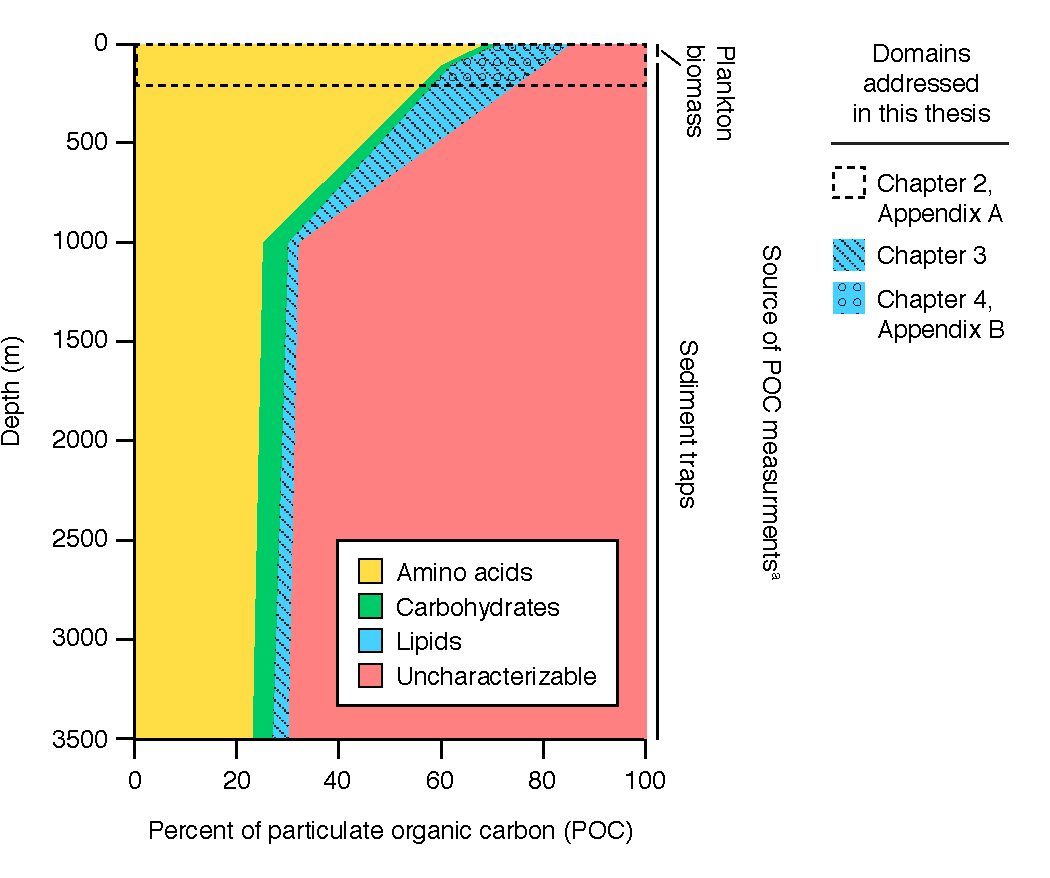
\includegraphics[width=0.75\textwidth]{Fig_1-1.pdf}
\captionsetup{font={footnotesize}}
\caption[Concept of the thesis in relation to the relative proportions of biochemicals in organic matter at different depths in the ocean.]{Percentage of particulate organic carbon in three of the four major classes of biochemicals, as determined in samples collected at various depths in the central equatorial Pacific by Wakeham et al. (1997). Depicted in red is the large fraction of organic matter that could not be characterized at the molecular level. Superimposed over the figure are the chemical and depth domains addressed by various chapters of the thesis. \textsuperscript{a} As reported by Wakeham et al. (1997). The sediment trap samples were collected at 105, 1000, and $\geq$ 3500 m.}
\label{fig:c1n1}
\end{figure}

\begin{figure}[!p]
\centering
\includegraphics[width=0.75\textwidth]{Fig_1-2.pdf}
\captionsetup{font={footnotesize}}
\caption[Schematic showing the major processes that ultimately remove sinking particle material in the mesopelagic ocean, as conceptualized in \autoref{chap2} of the thesis.]{Schematic showing the major processes that ultimately remove sinking particle material in the mesopelagic ocean, as conceptualized in \autoref{chap2} of the thesis (Collins et al., 2015). Also shown are the accompanying first-order rate constants ($k$; units of day$^{-1}$) through which we represent these attenuation processes in the model described in that chapter. Arrow a, in magenta: Respiration of particle material by particle-attached heterotrophic bacteria ($k_{R}$, which we calculate from direct measurements). We use a single rate constant ($k_{S,D,Z}$) in our model sensitivity analyses to account for the other processes (arrows b-e), which we did not directly observe. $k_{S,D,Z}$ represents the fraction of particle flux attenuation that cannot be attributed to direct respiration by particle-attached bacteria. Arrow b, in orange: Enzymatic solubilization or mechanical disaggregation of particle material by attached bacteria. This process transfers organic matter to the dissolved or suspended phases in the surrounding water column, where it can then be metabolized by free-living bacterial communities (arrows f and g). Arrows c-e, in green: Particle flux attenuation processes attributable to zooplankton, including (arrow c) mechanical disaggregation (e.g., ``sloppy feeding''), (arrow d) egestion or excretion, or (arrow e) direct respiration of material to carbon dioxide. Disaggregation and excretion can transfer particle material to the dissolved or suspended phases; egestion of smaller fecal pellets can also transfer material to the suspended organic matter pool. Our interpretation of the sensitivity analysis results was informed by additional direct observations of arrow g.\\\\\tiny{Reproduced with permission from:\\\\Collins, J. R., B. R. Edwards, K. Thamatrakoln, J. E. Ossolinski, G. R. DiTullio, K. D. Bidle, S. C. Doney, and B. A. S. Van Mooy. 2015. The multiple fates of sinking particles in the North Atlantic Ocean. \emph{Global Biogeochemical Cycles} \emph{29}:1471-1494; doi:10.1002/2014GB005037\\\\\copyright 2015 American Geophysical Union}}
\label{fig:c1n2}
\end{figure}

First, in \autoref{chap2}, I sought to determine the relative contribution to particle flux attenuation by respiration compared to the other major biological and mechanical processes that progressively remove sinking particles with depth (\autoref{fig:c1n2}). I first present measurements collected at six stations in North Atlantic basin of sinking particulate carbon fluxes, water column bacterial production and respiration rates, and specific respiration rates on sinking particle material. I then calculate substrate-specific respiration rates on sinking particles, bacterial growth efficiencies (BGE) both in the water column and on sinking particle material, and depth-integrated estimates of water column BP and respiration for the upper mesopelagic zone (50 to 150 m). Finally, I apply the measurements of particulate organic carbon (POC) fluxes and substrate-specific respiration in a series of sensitivity analyses of a simple, yet mechanistic model of particle flux attenuation. Observational data and the results of these sensitivity analyses are combined to (1) constrain the relative contribution to particle flux attenuation by particle-attached microbial respiration compared to other processes and (2) determine how differences in the average sinking speed of marine particles affect this partitioning.

In \autoref{chap3}, I present a new software package and computational strategy for discovering lipid, oxylipin, and oxidized lipid biomarkers in large volumes of high-resolution, accurate-mass HPLC-ESI-MS lipid data. I was inspired in developing the software by the need for new computational approaches to parse the increasingly complex dataset that are generated in metabolomics and lipidomics studies (Cajka and Fiehn, 2016; Prosser et al., 2014). Lipid and Oxylipin Biomarker Screening through Adduct Hierarchy Sequences, or LOBSTAHS, is centered around a novel screening methodology that exploits the unique tendency of lipids to form adduct ions in consistent, diagnostic patterns of abundance that remain relatively consistent across sample types. Using lipid data from cultures of a mutant strain of a marine diatom (\emph{Phaeodactylum tricornutum}) designed for studies of oxidative stress (van Creveld et al., 2015), LOBSTAHS is applied in \autoref{chap3} to resolve conflicting compound assignments, examine differential expression of compounds across experimental treatments, discover and identify potential oxidized intact polar lipid (ox-IPL) and oxylipin biomarkers, and identify potential isomers and isobars. In the experimental dataset, a stress response is induced in the \emph{P. tricornutum} by treating the cultures with hydrogen peroxide (H$_2$O$_2$), a reactive oxygen species (ROS) that can be generated both biologically (e.g., as a consequence of metabolic activity) and abiotically (e.g., via photochemical reactions). H$_2$O$_2$ represents a persistent source of stress in many marine ecosystems.

\begin{figure}[!th]
\centering
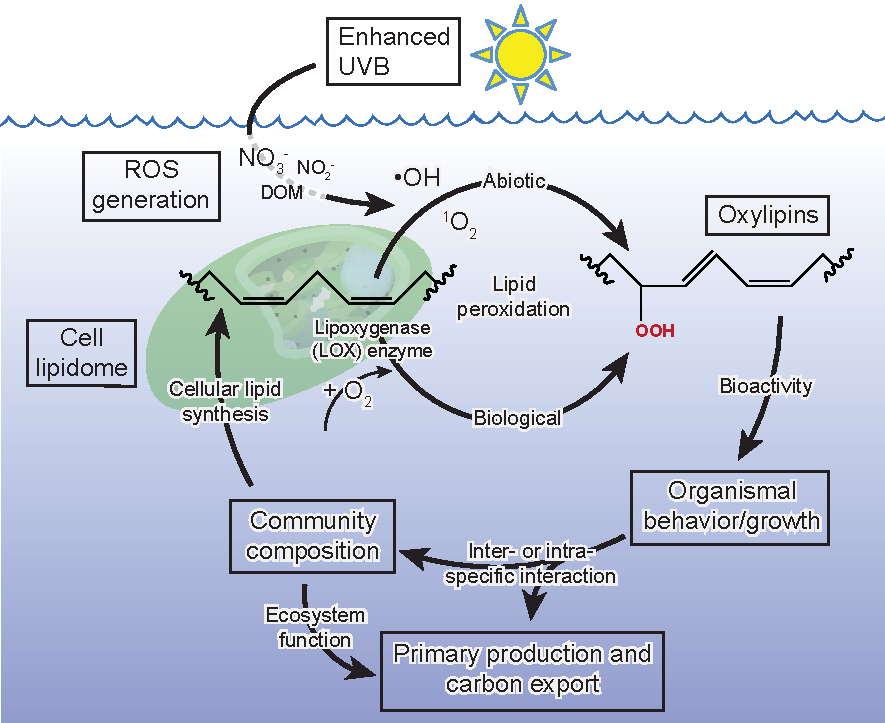
\includegraphics[width=1\textwidth]{Fig_1-3.pdf}
\captionsetup{font={footnotesize}}
\caption[Schematic illustrating the mechanisms through which oxidized lipids and oxylipins can be generated marine ecosystems, and the relationships between lipid peroxidation and several major biogeochemical and ecological processes.]{Schematic illustrating the mechanisms through which oxidized lipids and oxylipins can be generated marine ecosystems, and the relationships between lipid peroxidation and several major biogeochemical and ecological processes. In \autoref{chap4}, this conceptual framework is applied to the study of lipid photooxidation in surface waters of the West Antarctic Peninsula.
}
\label{fig:c1n3}
\end{figure}

In \autoref{chap4}, I explore the mechanisms and biogeochemical significance of lipid photooxidation in coastal surface waters of the West Antarctic Peninsula. The research in \autoref{chap4} was motivated by a paucity of information about the potentially complex relationships between ecosystem processes and the photochemical production of oxidized lipids and oxylipins induced by ultraviolet radiation (\autoref{fig:c1n3}). I combine results from experiments in a model liposome system with diverse environmental data --- including high-resolution, accurate-mass HPLC-ESI-MS analysis of lipid samples and in situ time-series measurements of ultraviolet irradiance --- to address several research objectives. By exposing liposomes to different light treatments under natural conditions, I sought to determine whether the photooxidation of intact polar diacylglycerols (IP-DAG; a broad class of membrane lipid) was dependent on molecular structure. Specifically, I hypothesized that a higher degree of unsaturation in the fatty acids of a particular IP-DAG would make it more amenable to photooxidation. As part of these experiments, I also investigated the effect of lipid photooxidation on natural communities of heterotrophic bacteria, and conversely, whether the presence of these bacteria would enhance apparent overall rates of lipid degradation. The diversity, quantities, and structures of various products of lipid photooxidation are queried by applying the data analysis methods described in \autoref{chap3} (Collins et al., 2016) to the HPLC-ESI-MS data from our liposome experiments. Using the same MS and data analysis methods, I also sought to characterize the lipidome of plankton from the WAP water column to determine what fraction of the particulate ($\geq$ 0.2 $\mu$m) lipid biomass would likely be amenable to degradation by photooxidation. Finally, I calculate broadband polychromatic apparent quantum yields (AQY) for photooxidation of IP-DAG under natural environmental conditions. These are applied to the water column lipid data and measurements of irradiance to estimate the significance of lipid photooxidation within the carbon cycle of the WAP ecosystem.

Finally, in \autoref{chap5}, I offer some new perspectives on the results and methods presented in the three main thesis chapters, and present some conclusions and directions for future research.

The thesis also contains several appendices: In \autoref{AppA}, I present a description and demonstration of the PHORCYS (PHOtosynthesis, Respiration, and Carbon-balance Yielding System), a new, incubation-based instrument that can be deployed in situ to determine rates of respiration and primary production in a wide range of marine and aquatic ecosystems. Development and testing of the PHORCYS was motivated by a surprising finding: Despite the attention that aerobic respiration has received relative to other processes that remineralize and degrade organic matter in the ocean, there are still far fewer total observations in the literature of respiration than primary production (\autoref{fig:c1n4}; le B. Williams and del Giorgio, 2005). Large discrepancies have also been observed between geochemical tracer and in vitro-based methods for measuring the net community productivity of marine ecosystems (le B. Williams et al., 2013). In \autoref{AppA}, respiration rate estimates from two versions of the PHORCYS are compared with estimates based a traditional method using Winkler titrations. A new method for estimating rates of error in metabolic rate measurements derived from dissolved oxygen time series is also presented. In \autoref{AppB}, I present some preliminary results from an experiment in which whole, unfiltered surface seawater samples from a site in the North Pacific Subtropical Gyre (NPSG) were exposed to different qualities of natural radiation during a series of shipboard incubations. The lipidomics pipeline described in \autoref{chap4} is applied to samples from the experiment to discover patterns and biomarkers of lipid photooxidation. The additional appendices (\autoref{AppC}, \autoref{AppD}, and \autoref{AppE}) contain supporting information, including supplementary figures and tables, for the main thesis chapters.

\begin{figure}[!th]
\centering
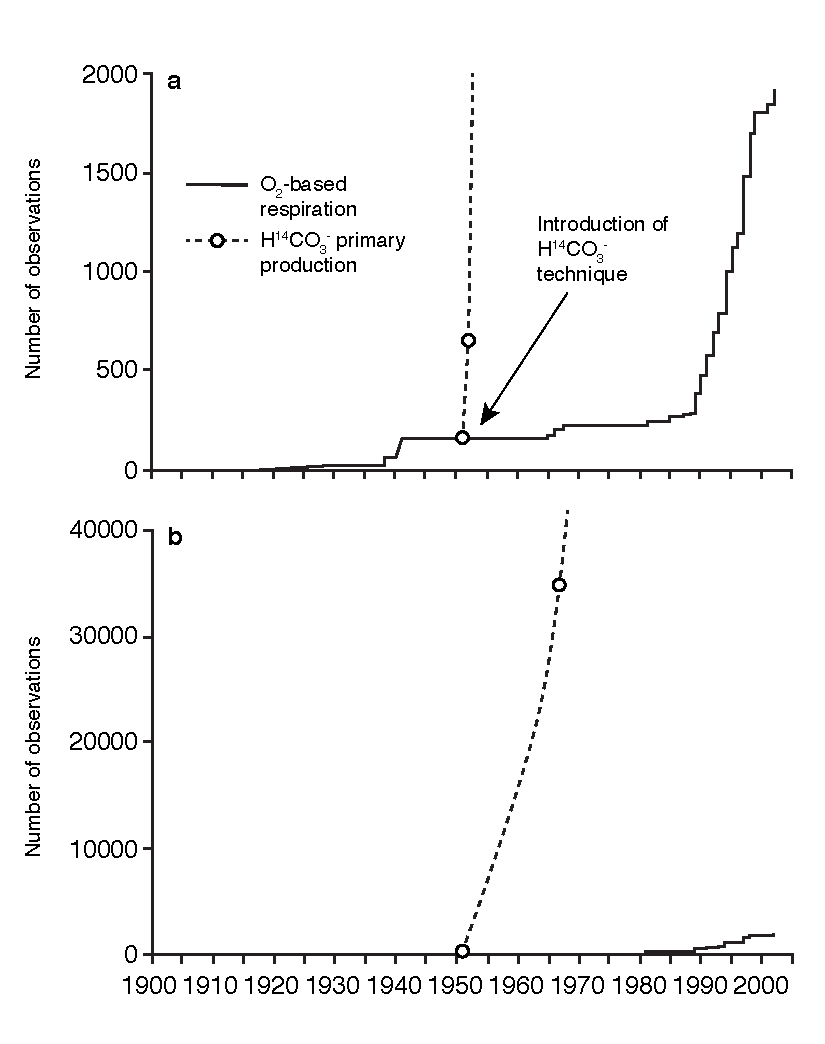
\includegraphics[width=.75\textwidth]{Fig_1-4.pdf}
\captionsetup{font={footnotesize}}
\caption[Cumulative estimate of the number of observations of aerobic respiration from measurements of dissolved oxygen and observations of primary production based on the H$^{14}$CO$_3^-$ method.]{Cumulative estimate of the number of observations of aerobic respiration from measurements of dissolved oxygen (solid line) and observations of primary production based on the H$^{14}$CO$_3^-$ method (dashed line). The figure is modified from Williams and del Giorgio (2005). Panel (a) shows the same data as panel (b), but with a 20-fold expansion of the \emph{y}-axis.}
\label{fig:c1n4}
\end{figure}

In preparing this thesis, I was keenly aware of a widely-held perception that geoscientists have been slow to adopt many of the core tenets of open science (McNutt et al., 2016). Accordingly, I have endeavored to make all data, software, and code required to reproduce the results in this thesis publicly available in open-source or non-proprietary formats; instructions can be found in designated sections at the end of each chapter, or in the corresponding supporting information. I sincerely apologize that some of my earlier computations (for \autoref{chap2}) were performed in MATLAB. MATLAB is a great product, but it costs a considerable amount of money for those who don't have access to a site license. With this caveat, I have hewed as closely as possible to the guidelines established by the \href{http://www.scientificpaperofthefuture.org/gpf/what-is-a-gpf}{Geoscience Papers of the Future Initiative} for provenance and data and software availability.
\clearpage
\begin{singlespace}
\section*{References}
\addtocounter{section}{1}
{\setlength{\parindent}{0pt}
Ar\'{i}stegui, J., C. M. Duarte, S. Agust\'{i}, M. Doval, X. A. \'{A}lvarez-Salgado,
and D. A. Hansell (2002), Dissolved organic carbon support of
respiration in the dark ocean, \emph{Science}, \emph{298}(5600),
1967-1967, doi:\href{http://dx.doi.org/10.1126/science.1076746}{10.1126/science.1076746}.

{\setlength{\parskip}{10pt}

Arrhenius, S. (1896), On the influence of carbonic acid in the air upon the temperature of the ground, \emph{London, Edinburgh and Dublin Philosophical Magazine and Journal of Science}, \emph{41}, 237-276.

Berner, R. A. (1981), A new geochemical classification of sedimentary
environments, \emph{Journal of Sedimentary Research}, \emph{51}(2),
359-365, doi:\href{http://dx.doi.org/10.1306/212f7c7f-2b24-11d7-8648000102c1865d}{10.1306/212f7c7f-2b24-11d7-8648000102c1865d}.

Broecker, W. S. (1983), The ocean, \emph{Scientific American}, \emph{249}, 146-161.

Cajka, T., and O. Fiehn (2016), Toward merging untargeted and targeted
methods in mass spectrometry-based metabolomics and lipidomics,
\emph{Analytical Chemistry}, \emph{88}(1), 524-545,
doi:\href{http://dx.doi.org/10.1021/acs.analchem.5b04491}{10.1021/acs.analchem.5b04491}.

Carlson, C. A., and H. W. Ducklow (1996), Growth of bacterioplankton and
consumption of dissolved organic carbon in the Sargasso Sea,
\emph{Aquatic Microbial Ecology}, \emph{10}(1), 69-85.

Chamberlin, T. C. (1898), The influence of great epochs of limestone formation upon the constitution of the atmosphere, \emph{Journal of Geology}, \emph{6}, 609-621.

Close, H. G., S. R. Shah, A. E. Ingalls, A. F. Diefendorf, E. L. Brodie,
R. L. Hansman, K. H. Freeman, L. I. Aluwihare, and A. Pearson (2013),
Export of submicron particulate organic matter to mesopelagic depth in
an oligotrophic gyre, \emph{Proceedings of the National Academy of Sciences of the United States of America}, \emph{110}(31),
12565-12570, doi:\href{http://dx.doi.org/10.1073/pnas.1217514110}{10.1073/pnas.121751411\\0}.

Collins, J. R., B. R. Edwards, K. Thamatrakoln, J. E. Ossolinski, G. R.
DiTullio, K. D. Bidle, S. C. Doney, and B. A. S. Van Mooy (2015), The
multiple fates of sinking particles in the North Atlantic Ocean,
\emph{Global Biogeochemical Cycles}, \emph{29}, 1471-1494,
doi:\href{http://dx.doi.org/10.1002/2014GB005037}{10.1002/2014GB005\\037}.

D. Krom, M., and R. A. Berner (1981), The diagenesis of phosphorus in a
nearshore marine sediment, \emph{Geochimica et Cosmochimica Acta},
\emph{45}(2), 207-216, doi:\href{http://dx.doi.org/10.1016/0016-7037(81)90164-2}{10.1016/0016-7037(81)90164-2}.

del Giorgio, P. A., and C. M. Duarte (2002), Respiration in the open
ocean, \emph{Nature}, \emph{420}(6914), 379-384.

del Giorgio, P. A., J. J. Cole, and A. Cimbleris (1997), Respiration
rates in bacteria exceed phytoplankton production in unproductive
aquatic systems, \emph{Nature}, \emph{385}(6612), 148-151.

Ducklow, H. W., and S. C. Doney (2013), What is the metabolic state of
the oligotrophic ocean? A debate, \emph{Annual Review of Marine Science}, \emph{5},
15.11--15.19, doi:\\\href{http://dx.doi.org/10.1146/annurev-marine-121211-172331}{10.1146/annurev-marine-121211-172331}.

Dugdale, R. C., and J. J. Goering (1967), Uptake of new and regenerated forms of nitrogen in primary productivity, \emph{Limnology \& Oceanography}, \emph{12}(2), 196-206.

Eppley, R. W., and B. J. Peterson (1979), Particulate organic matter flux and planktonic new production in the deep ocean, \emph{Nature}, \emph{282}(5740), 677-680.

Falkowski, P. G. (2014), Biogeochemistry of primary production in the
sea, in \emph{Treatise on Geochemistry (Second Edition)}, edited by K.
K. Turekian, pp. 163-187, Elsevier, Oxford,
doi:\href{http://dx.doi.org/10.1016/B978-0-08-095975-7.00805-6}{10.1016/B978-0-08-095975-7.00805-6}.

Giering, S. L. C., et al. (2014), Reconciliation of the carbon budget in
the ocean's twilight zone, \emph{Nature}, \emph{507}(7493), 480-483,
doi:\href{http://dx.doi.org/10.1038/nature13123}{10.1038/nature13123}.

Gorham, E. (1991), Biogeochemistry: its origins and development, \emph{Biogeochemistry}, \emph{13}(3), 199-239.

Grossart, H. P., A. Engel, C. Arnosti, C. L. De La Rocha, A. E. Murray,
and U. Passow (2007), Microbial dynamics in autotrophic and
heterotrophic seawater mesocosms. III. Organic matter fluxes,
\emph{Aquatic Microbial Ecology}, \emph{49}(2), 143-156,
doi:\href{http://dx.doi.org/10.3354/ame01140}{10.3354/ame01140}.

Hedges, J. I., J. A. Baldock, Y. Gelinas, C. Lee, M. Peterson, and S. G.
Wakeham (2001), Evidence for non-selective preservation of organic
matter in sinking marine particles, \emph{Nature}, \emph{409}(6822),
801-804.

Hunter, J. E., M. J. Frada, H. F. Fredricks, A. Vardi, and B. A. S. Van
Mooy (2015), Targeted and untargeted lipidomics of \emph{Emiliania huxleyi}
viral infection and life cycle phases highlights molecular biomarkers of
infection, susceptibility, and ploidy, \emph{Frontiers in Marine
Science}, \emph{2}, doi:\href{http://dx.doi.org/10.3389/fmars.2015.00081}{10.3389/fmars.2015.00081}.

Keil, R. G., D. B. Montlucon, F. G. Prahl, and J. I. Hedges (1994),
Sorptive preservation of labile organic matter in marine sediments,
\emph{Nature}, \emph{370}(6490), 549-552.

Kieber, D. J., J. McDaniel, and K. Mopper (1989), Photochemical source
of biological substrates in sea water: implications for carbon cycling,
\emph{Nature}, \emph{341}(6243), 637-639.

Killops, S. D., and V. J. Killops (2005), \emph{An Introduction to
Organic Geochemistry}, 2nd ed., 408 pp., Wiley-Blackwell, New York.

McNutt, M., K. Lehnert, B. Hanson, B. A. Nosek, A. M. Ellison, and J. L.
King (2016), Liberating field science samples and data, \emph{Science},
\emph{351}(6277), 1024-1026, doi:\href{http://dx.doi.org/10.1126/science.aad7048}{10.1126/science.a\\ad7048}.

Middelburg, J. J. (1989), A simple rate model for organic matter
decomposition in marine sediments, \emph{Geochimica et Cosmochimica Acta},
\emph{53}(7), 1577-1581, doi:\href{http://dx.doi.org/10.1016/0016-7037(89)90239-1}{10.1016/0016-7037(89)90239-1}.

Miller, W. L., and R. G. Zepp (1995), Photochemical production of
dissolved inorganic carbon from terrestrial organic matter: Significance
to the oceanic organic carbon cycle, \emph{Geophysical Research Letters},
\emph{22}(4), 417-420, doi:\href{http://dx.doi.org/10.1029/94GL03344}{10.1029/94GL03344}.

Mopper, K., and D. J. Kieber (2002), Photochemistry and the cycling of
carbon, sulfur, nitrogen and phosphorous, in \emph{Biogeochemistry of
Marine Dissolved Organic Matter}, edited by D. A. Hansell and C. A.
Carlson, pp. 455-489, Academic Press, New York.

Mopper, K., X. Zhou, R. J. Kieber, D. J. Kieber, R. J. Sikorski, and R.
D. Jones (1991), Photochemical degradation of dissolved organic carbon
and its impact on the oceanic carbon cycle, \emph{Nature},
\emph{353}(6339), 60-62.

Mottl, M. J., and H. Elderfield (2014), Volume editor's introduction, in \emph{Treatise on Geochemistry (Second Edition)}, edited by K. K. Turekian, pp. xxiii-xxv, Elsevier, Oxford, doi:\href{http://dx.doi.org/10.1016/B978-0-08-095975-7.09985-X}{10.1016/B978-0-08-095975-7.09985-X}.

Pearson, A. (2014), Lipidomics for geochemistry, in \emph{Treatise on
Geochemistry}, edited by H. D. Holland and K. K. Turekian, pp. 291-336,
Elsevier, Oxford.

Perrault, P. (1674), \emph{De l'origine des fontaines} (\emph{On the Origin of Springs}, translated by Hafner, 1966).

Petsch, S. T. (2014), Weathering of organic carbon, in \emph{Treatise on
Geochemistry (Second Edition)}, edited by K. K. Turekian, pp. 217-238,
Elsevier, Oxford, doi:\href{http://dx.doi.org/10.1016/B978-0-08-095975-7.01013-5}{10.1016/B978-0-08-095975-7.01013-5}.

Ploug, H., and H.-P. Grossart (1999), Bacterial production and
respiration in suspended aggregates --- a matter of the incubation
method, \emph{Aquatic Microbial Ecology}, \emph{20}, 21-29.

Prosser, G. A., G. Larrouy-Maumus, and L. P. de Carvalho (2014),
Metabolomic strategies for the identification of new enzyme functions
and metabolic pathways, \emph{EMBO Reports}, \emph{15}(6), 657-669,
doi:\href{http://dx.doi.org/10.15252/embr.201338283}{10.15252/embr.201338283}.

Rontani, J.-F., B. Charriere, A. Forest, S. Heussner, F. Vaultier, M.
Petit, N. Delsaut, L. Fortier, and R. Sempere (2012), Intense
photooxidative degradation of planktonic and bacterial lipids in sinking
particles collected with sediment traps across the Canadian Beaufort
Shelf (Arctic Ocean), \emph{Biogeosciences}, \emph{9}(11), 4787-4802,
doi:\href{http://dx.doi.org/10.5194/Bg-9-4787-2012}{10.5194/Bg-9-4787-2012}.

Rontani, J.-F., B. Charriere, M. Petit, F. Vaultier, H. J. Heipieper, H.
Link, G. Chaillou, and R. Sempere (2012), Degradation state of organic
matter in surface sediments from the Southern Beaufort Sea: a lipid
approach, \emph{Biogeosciences}, \emph{9}(9), 3513-3530,
doi:\href{http://dx.doi.org/10.5194/Bg-9-3513-2012}{10.5194/Bg-9-3513-2012}.

Stemmann, L., G. A. Jackson, and G. Gorsky (2004), A vertical model of
particle size distributions and fluxes in the midwater column that
includes biological and physical processes---Part II: application to a
three year survey in the NW Mediterranean Sea, \emph{Deep Sea Research
Part I: Oceanographic Research Papers}, \emph{51}(7), 885-908,
doi:\href{http://dx.doi.org/10.1016/j.dsr.2004.03.002}{10.1016/j.dsr.2004.03.002}.

Sturt, H. F., R. E. Summons, K. Smith, M. Elvert, and K. U. Hinrichs
(2004), Intact polar membrane lipids in prokaryotes and sediments
deciphered by high-performance liquid chromatography/electrospray
ionization multistage mass spectrometry - new biomarkers for
biogeochemistry and microbial ecology, \emph{Rapid Communications in Mass Spectrometry}, \emph{18}(6), 617-628, doi:\href{http://dx.doi.org/10.1002/rcm.1378}{10.1002/rcm.1378}.

Sundquist, E. T., and K. V. Ackerman (2014), The geologic history of the carbon cycle, in \emph{Treatise on Geochemistry (Second Edition)}, edited by K. K. Turekian, pp. 361-398, Elsevier, Oxford, doi:\href{http://dx.doi.org/10.1016/B978-0-08-095975-7.00809-3}{10.1016/B978-0-08-095975-7.00809-3}.

van Creveld, S. G., S. Rosenwasser, D. Schatz, I. Koren, and A. Vardi
(2015), Early perturbation in mitochondria redox homeostasis in response
to environmental stress predicts cell fate in diatoms, \emph{The ISME Journal},
\emph{9}(2), 385-395, doi:\href{http://dx.doi.org/10.1038/ismej.2014.136}{10.1038/ismej.2014.136}.

Van Mooy, B. A. S., G. Rocap, H. F. Fredricks, C. T. Evans, and A. H.
Devol (2006), Sulfolipids dramatically decrease phosphorus demand by
picocyanobacteria in oligotrophic marine environments, \emph{Proceedings of the National Academy of Sciences of the United States of America}, \emph{103}(23), 8607-8612, doi:\href{http://dx.doi.org/10.1073/pnas.0600540103}{10.1073/pnas.0600540103}.

Van Mooy, B. A. S., et al. (2009), Phytoplankton in the ocean use
non-phosphorus lipids in response to phosphorus scarcity, \emph{Nature},
\emph{458}(7234), 69-72.

Vardi, A., L. Haramaty, B. A. Van Mooy, H. F. Fredricks, S. A. Kimmance,
A. Larsen, and K. D. Bidle (2012), Host-virus dynamics and subcellular
controls of cell fate in a natural coccolithophore population,
\emph{Proceedings of the National Academy of Sciences of the United
States of America}, \emph{109}(47), 19327-19332,
doi:\href{http://dx.doi.org/10.1073/pnas.1208895109}{10.1073/pnas.1208895109}.

Vernadsky, V. I. (1924), \emph{La G\'{e}ochimie}, Alcan, Paris.

Volk, T., and M. I. Hoffert (1985), Ocean carbon pumps: Analysis of relative strengths and efficiencies in ocean-driven atmospheric CO2 changes, in \emph{The Carbon Cycle and Atmospheric CO2: Natural Variations Archean to Present}, edited by E. T. Sundquist and W. S. Broecker, pp. 99-110, AGU, Washington, DC, doi:\href{http://dx.doi.org/10.1029/GM032p0099}{10.1029/GM032p0099}.

Wakeham, S. G., J. I. Hedges, C. Lee, M. L. Peterson, and P. J. Hernes
(1997), Compositions and transport of lipid biomarkers through the water
column and surficial sediments of the equatorial Pacific Ocean,
\emph{Deep Sea Research Part II: Topical Studies in Oceanography}, \emph{44}(9-10), 2131-2162,
doi:\href{http://dx.doi.org/10.1016/s0967-0645(97)00035-0}{10.1016/s0967-0645(97)00035-0}.

Wakeham, S. G., C. Lee, J. I. Hedges, P. J. Hernes, and M. J. Peterson
(1997), Molecular indicators of diagenetic status in marine organic
matter, \emph{Geochimica et Cosmochimica Acta}, \emph{61}(24), 5363-5369,
doi:\href{http://dx.doi.org/10.1016/S0016-7037(97)00312-8}{10.1016/S0016-7037(97)00312-8}.

Williams, P. J. le B. (1998), The balance of plankton respiration and
photosynthesis in the open oceans, \emph{Nature}, \emph{394}(6688),
55-57.

Williams, P. J. le B., and P. del Giorgio (2005), Respiration in aquatic
ecosystems: history and background, in \emph{Respiration in Aquatic
Ecosystems}, edited by P. del Giorgio and P. J. le B. Williams, Oxford
University Press, New York.

Williams, P. J. le B., P. D. Quay, T. K. Westberry, and M. J. Behrenfeld
(2013), The oligotrophic ocean is autotrophic, \emph{Annual Review of Marine Science}, \emph{5}, 16.11-16.15, doi:\href{http://dx.doi.org/10.1146/annurev-marine-121211-172335}{10.1146/\\annurev-marine-121211-172335}.

Zafiriou, O. C., S. S. Andrews, and W. Wang (2003), Concordant estimates
of oceanic carbon monoxide source and sink processes in the Pacific
yield a balanced global ``blue-water'' CO budget, \emph{Global
Biogeochemical Cycles}, \emph{17}(1), 1015, doi:\href{http://dx.doi.org/10.1029/2001GB001638}{10.1029/2001GB001638}.}}
\end{singlespace}